\documentclass[conference]{IEEEtran}
\usepackage[utf8]{inputenc}
\usepackage[T1]{fontenc}
\usepackage[brazil]{babel}
\usepackage{graphicx}
\usepackage{booktabs}
\usepackage{amsmath}
\usepackage{array}
\usepackage[hidelinks]{hyperref}
\usepackage{cite}

\renewcommand{\IEEEkeywordsname}{Palavras-chave}

\begin{document}

\title{Detecção de Tumores Cerebrais em Imagens de Ressonância Magnética por \textit{Transfer Learning} com Validação Cruzada por Grupos}

\author{
\IEEEauthorblockN{Matheus Lemes Amaral}
\IEEEauthorblockA{\textit{FGA0261 --- Inteligência Artificial II}\\
Universidade de Brasília (UnB)\\
Brasília, Brasil\\
Matrícula: 241031852}
\and
\IEEEauthorblockN{Eduardo Jesus Dal Pizzol}
\IEEEauthorblockA{\textit{FGA0261 --- Inteligência Artificial II}\\
Universidade de Brasília (UnB)\\
Brasília, Brasil\\
Matrícula: 251008114}
}

\maketitle

\begin{abstract}
Conjuntos públicos de ressonância magnética (RM) cerebral costumam ser pequenos e conter imagens repetidas. Este trabalho classifica fatias de RM em ``com tumor'' e ``sem tumor'' no conjunto público \textit{Brain MRI Images for Brain Tumor Detection} (253 imagens), após remover 25 cópias idênticas e agrupar quase-duplicatas por \textit{hash} perceptual. Uma ResNet-18 pré-treinada no ImageNet é comparada a uma CNN treinada do zero, e quatro configurações de treino são comparadas por validação cruzada estratificada por grupos (5 \textit{folds} $\times$ 3 sementes). A ResNet-18 obteve AUC média de $0{,}917$ a $0{,}923$ nas três melhores configurações, e nenhuma diferença pareada em relação à configuração inicial se afastou de zero (melhor caso: $+0{,}005$, IC 95\% $[-0{,}010;\,0{,}021]$). No teste (34 imagens), a melhor configuração errou uma imagem (acurácia $0{,}971$, AUC $0{,}989$), contra AUC de $0{,}733$ da CNN sem pré-treino. Sem identificação de paciente nem validação externa, os resultados são exploratórios e não indicam uso clínico.
\end{abstract}

\begin{IEEEkeywords}
aprendizado profundo, \textit{transfer learning}, ressonância magnética, tumor cerebral, validação cruzada.
\end{IEEEkeywords}

\section{Introdução}

A ressonância magnética é o principal exame de imagem para detectar e acompanhar tumores cerebrais, e sua leitura depende da experiência do examinador. Redes neurais convolucionais (CNNs) já foram aplicadas à classificação de tumores em RM~\cite{swati2019brain,deepak2019brain} e podem apoiar a triagem ao sinalizar exames suspeitos para revisão, sem substituir o diagnóstico.

Os conjuntos públicos mais acessíveis, porém, são pequenos e podem conter a mesma imagem mais de uma vez; nesse caso, a divisão aleatória coloca cópias de um exame no treino e no teste, e o desempenho relatado fica inflado por vazamento de dados~\cite{kapoor2023leakage}, problema identificado em mais da metade dos estudos de CNN em RM revisados por Wen \textit{et al.}~\cite{wen2020alzheimer}. Além disso, comparações entre configurações costumam relatar uma única divisão, sem incerteza.

Este trabalho compara uma ResNet-18~\cite{he2016resnet} pré-treinada a uma CNN treinada do zero e avalia quatro configurações de treino com deduplicação, divisão por grupos de quase-duplicatas e teste usado uma única vez, ao final. São investigadas três questões de pesquisa:
\begin{itemize}
\item \textbf{QP1:} o \textit{transfer learning} do ImageNet melhora a classificação em relação a uma CNN treinada do zero com tão poucos dados?
\item \textbf{QP2:} ajustes de agendamento da taxa de aprendizado, \textit{weight decay} e congelamento inicial alteram a discriminação quando avaliados por validação cruzada por grupos?
\item \textbf{QP3:} um limiar escolhido na validação para garantir alta sensibilidade compensa em relação ao limiar fixo de 0,5?
\end{itemize}
A Seção~II apresenta a fundamentação; a III, a metodologia; a IV, os resultados; a V, a discussão e as ameaças à validade; e a VI conclui.

\section{Fundamentação e Trabalhos Relacionados}

No \textit{transfer learning}, uma rede pré-treinada em uma base grande, como o ImageNet~\cite{deng2009imagenet}, é reaproveitada em outra tarefa. As primeiras camadas aprendem filtros genéricos, como bordas e texturas, e as últimas, padrões específicos da tarefa original~\cite{yosinski2014transferable}; por isso, o \textit{fine-tuning} costuma funcionar com poucas imagens médicas. A ResNet~\cite{he2016resnet} introduziu conexões residuais, em que cada bloco aprende uma correção $F(x)$ somada à entrada $x$, o que permite treinar redes profundas sem degradação; a ResNet-18, com a cabeça de uma saída usada aqui, tem 11,2M de parâmetros.

Com classes desbalanceadas, a acurácia favorece a classe majoritária; por isso, relatam-se também sensibilidade, especificidade, F1 e a AUC ROC, que independe do limiar. Quando há várias imagens do mesmo exame, a validação precisa manter cada grupo inteiro em uma única partição, como faz a validação cruzada estratificada por grupos~\cite{pedregosa2011sklearn}.

Swati \textit{et al.}~\cite{swati2019brain} ajustaram uma CNN pré-treinada bloco a bloco para classificar glioma, meningioma e tumor hipofisário em RM ponderada em T1 com contraste, com acurácia média de 94,8\% em validação cruzada de 5 \textit{folds}, e Deepak e Ameer~\cite{deepak2019brain} usaram atributos de uma GoogLeNet pré-treinada no mesmo problema de três classes. Para segmentação, o BRATS~\cite{menze2015brats} estabeleceu um \textit{benchmark} multimodal de gliomas. Diferentemente desses trabalhos, este estudo usa um conjunto binário pequeno e de fonte única e concentra-se no protocolo: deduplicação, divisão por grupos e comparação pareada de configurações com incerteza.

\section{Metodologia}

\begin{figure}[t]
\centering
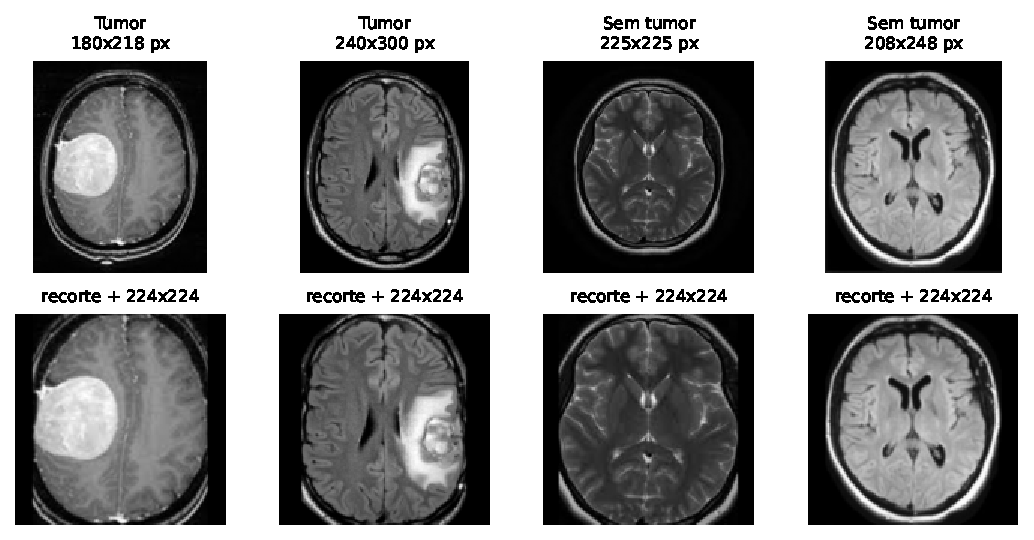
\includegraphics[width=0.92\columnwidth]{fig_preprocess.pdf}
\caption{Exemplos do conjunto original (acima), com resoluções variadas, e o resultado do recorte do crânio e da padronização em $224\times224$ (abaixo).}
\label{fig:pre}
\end{figure}

\begin{table}[t]
\centering
\caption{Protocolo experimental.}
\label{tab:protocolo}
\footnotesize
\renewcommand{\arraystretch}{1.05}
\begin{tabular}{@{}p{1.5cm}p{6.25cm}@{}}
\toprule
Aspecto & Configuração \\
\midrule
Dados & \textit{Brain MRI Images for Brain Tumor Detection}~\cite{kaggle2019brain}; 253 imagens (155 tumor, 98 sem tumor) \\
Amostra & 228 imagens únicas (25 cópias removidas); 216 grupos de quase-duplicatas (\textit{dHash} $8\times8$) \\
Rótulos & Binário por imagem: tumor / sem tumor \\
Divisão & 70/15/15 por grupo, estratificada por classe (semente 42): 160/34/34 imagens \\
Entrada & Recorte do crânio, \textit{padding} quadrado, $224\times224$, normalização ImageNet \\
Aumento (treino) & Recorte aleatório (escala 0,85--1), espelhamento horizontal, rotação $\pm15^\circ$, brilho e contraste $\pm20\%$ \\
Modelos & ResNet-18 (11,2M; pesos ImageNet) e CNN simples (1,2M; do zero); \textit{dropout} 0,3 + 1 \textit{logit} \\
Perda & Entropia cruzada binária com peso positivo $n_{\text{sem}}/n_{\text{tumor}}$ \\
Otimização & AdamW~\cite{loshchilov2019adamw}; taxa $10^{-4}$ ($10^{-3}$ na CNN simples); lote 32; cosseno~\cite{loshchilov2017sgdr}; precisão mista bf16 \\
Treino & Até 60 ou 25 épocas; parada antecipada pela perda de validação (paciência 15); GPU A100 80 GB \\
Seleção & Validação cruzada por grupos, 5 \textit{folds} $\times$ 3 sementes; maior AUC média (critério fixado antes) \\
Limiar & 0,5 fixo; alternativa: maior limiar com sensibilidade $\ge0{,}95$ na validação interna \\
Incerteza & \textit{Bootstrap} sobre as imagens de teste (2.000 repetições), IC 95\%~\cite{efron1993bootstrap} \\
\bottomrule
\end{tabular}
\end{table}

\subsection{Dados e rótulos}

Utilizou-se o conjunto público \textit{Brain MRI Images for Brain Tumor Detection}~\cite{kaggle2019brain}, com 253 fatias axiais de RM cerebral em duas pastas: 155 com tumor e 98 sem tumor. As imagens são heterogêneas: há 184 resoluções diferentes e quatro modos de cor (RGB, tons de cinza, RGBA e paleta), e não há metadados de paciente, sequência ou equipamento. A unidade de análise é a imagem, e a tarefa é binária. A inspeção dos arquivos revelou 25 cópias idênticas byte a byte de outras imagens e outros pares quase idênticos.

\subsection{Pré-processamento e divisão}

Cada imagem foi convertida para tons de cinza e as 25 cópias foram descartadas, restando 228 imagens. Para capturar quase-duplicatas, calculou-se um \textit{hash} de diferença (\textit{dHash}) de 64 bits: a imagem é reduzida a $9\times8$ pixels e cada bit indica se um pixel é mais claro que o vizinho da direita. Imagens com o mesmo \textit{hash} foram unidas em 216 grupos, e um grupo nunca é dividido entre partições.

O crânio foi isolado por filtro gaussiano $5\times5$, limiarização em 45, erosão e dilatação, e a imagem foi recortada na caixa do maior contorno externo. O recorte recebeu bordas pretas até ficar quadrado, o que preserva a proporção, e foi redimensionado para $224\times224$ pixels (Fig.~\ref{fig:pre}). Grupos inteiros de cada classe foram então sorteados para treino, validação e teste na proporção 70/15/15 (Tabela~\ref{tab:protocolo}). O aumento de dados foi aplicado só no treino, sem espelhamento vertical, que inverteria a anatomia.

\subsection{Modelos e treinamento}

As duas redes têm uma saída única (\textit{logit}), com a sigmoide aplicada dentro da perda. A ResNet-18 foi carregada do torchvision com pesos do ImageNet, e a última camada foi substituída por \textit{dropout} e uma camada linear; toda a rede foi ajustada. A CNN simples tem quatro blocos de duas convoluções $3\times3$ com \textit{batch normalization}, ReLU e \textit{max pooling} (32 a 256 canais), seguidos de \textit{pooling} médio global.

Partindo do primeiro experimento (\texttt{baseline}), três configurações acrescentam, cada uma, uma mudança à anterior (Tabela~\ref{tab:configs}). No \texttt{baseline}, o cosseno foi dimensionado para 60 épocas, mas a parada antecipada encerrou o treino na época 23, e a taxa de aprendizado ainda estava em 96\% do valor inicial na melhor época; $10^{-4}$ é um \textit{weight decay} fraco para o AdamW; e treinar a rede inteira desde o início deixa a cabeça aleatória propagar gradientes ruidosos para as camadas pré-treinadas.

\begin{table}[t]
\centering
\caption{Configurações de treino comparadas (ResNet-18).}
\label{tab:configs}
\footnotesize
\setlength{\tabcolsep}{2.5pt}
\begin{tabular}{@{}lccccc@{}}
\toprule
Configuração & Épocas & \textit{Warmup} & \textit{W. decay} & Só cabeça & LR cabeça \\
\midrule
\texttt{baseline} & 60 & 0 & $10^{-4}$ & 0 & $10^{-4}$ \\
\texttt{schedule} & 25 & 2 & $10^{-4}$ & 0 & $10^{-4}$ \\
\texttt{schedule\_wd} & 25 & 2 & $5\cdot10^{-2}$ & 0 & $10^{-4}$ \\
\texttt{sched.\_wd\_freeze} & 25 & 2 & $5\cdot10^{-2}$ & 3 & $10^{-3}$ \\
\bottomrule
\end{tabular}
\end{table}

\subsection{Avaliação e inferência}

As configurações foram comparadas por validação cruzada usando só as 194 imagens de treino e validação. Para cada semente (42, 43 e 44), as imagens foram divididas em 5 \textit{folds} com \texttt{StratifiedGroupKFold}~\cite{pedregosa2011sklearn}, que preserva a proporção das classes e mantém cada grupo em um único \textit{fold}. Em cada \textit{fold}, o modelo treina em quatro partes, com validação interna por grupos (15\%) para a parada antecipada e o limiar, e é avaliado na quinta (36 a 41 imagens). São 15 execuções por configuração, com as mesmas sementes e \textit{folds} para todas; a comparação com o \texttt{baseline} é pareada, com IC 95\% pela distribuição $t$ sobre as 15 diferenças.

A configuração vencedora e o \texttt{baseline} foram retreinados na divisão original e avaliados uma única vez no teste, com IC 95\% por \textit{bootstrap}. Hiperparâmetros, épocas e limiares foram definidos sem acesso ao teste. Código, divisão e predições estão em \url{https://github.com/1emes/MRI-segmentation}.

\begin{figure*}[t]
\centering
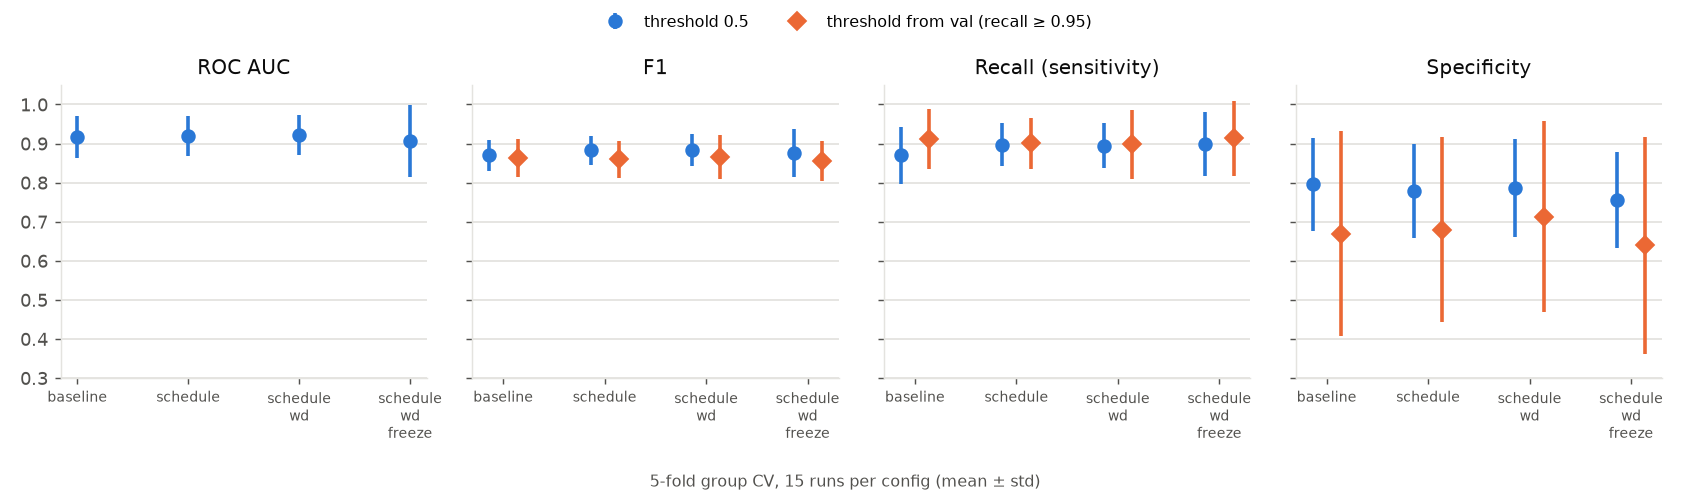
\includegraphics[width=0.84\textwidth]{../results/cv/cv_comparison.png}
\caption{Validação cruzada por grupos (média $\pm$ desvio de 15 execuções por configuração) com limiar fixo de 0,5 (círculos) e limiar escolhido na validação interna para sensibilidade $\ge0{,}95$ (losangos).}
\label{fig:cv}
\end{figure*}

\section{Resultados}

\subsection{\textit{Transfer learning} versus treino do zero}

No primeiro experimento (divisão única, configuração \texttt{baseline}), a ResNet-18 pré-treinada superou a CNN treinada do zero em todas as métricas de teste (Tabela~\ref{tab:arch}). A CNN simples classificou quase metade das imagens saudáveis como tumor (especificidade 0,538) e obteve AUC de 0,733, com intervalo que vai de 0,51 a 0,92; a ResNet-18 errou três das 34 imagens.

\begin{table}[t]
\centering
\caption{Teste (34 imagens): ResNet-18 pré-treinada vs.\ CNN do zero [IC 95\% por \textit{bootstrap}].}
\label{tab:arch}
\footnotesize
\setlength{\tabcolsep}{3pt}
\begin{tabular}{@{}lccc@{}}
\toprule
Métrica & Trivial\textsuperscript{a} & ResNet-18 & CNN simples \\
\midrule
Acurácia & 0,618 & \textbf{0,912} [0,79; 1,00] & 0,765 [0,62; 0,91] \\
Precisão & 0,618 & \textbf{0,909} [0,76; 1,00] & 0,760 [0,58; 0,92] \\
Sensibilidade & 1,000 & \textbf{0,952} [0,84; 1,00] & 0,905 [0,76; 1,00] \\
Especificidade & 0,000 & \textbf{0,846} [0,63; 1,00] & 0,538 [0,25; 0,80] \\
F1 & 0,764 & \textbf{0,930} [0,84; 1,00] & 0,826 [0,68; 0,93] \\
AUC & 0,500 & \textbf{0,971} [0,90; 1,00] & 0,733 [0,51; 0,92] \\
VN/FP/FN/VP & 0/13/0/21 & 11/2/1/20 & 7/6/2/19 \\
\bottomrule
\multicolumn{4}{@{}l@{}}{\scriptsize \textsuperscript{a}Prever todas as imagens como tumor. Prevalência no teste: 62\%.}
\end{tabular}
\end{table}

\subsection{Configurações de treino na validação cruzada}

A Tabela~\ref{tab:cv} e a Fig.~\ref{fig:cv} resumem as 15 execuções de cada configuração. As três primeiras ficaram entre 0,917 e 0,923 de AUC, e nenhuma diferença pareada em relação ao \texttt{baseline} teve intervalo que excluísse zero: a melhor, \texttt{schedule\_wd}, ganhou $+0{,}005$ (IC $[-0{,}010;\,0{,}021]$), com 9 vitórias, 1 empate e 5 derrotas. Congelar o \textit{backbone} nas três primeiras épocas reduziu a AUC em $0{,}011$ e quase dobrou o desvio entre \textit{folds} ($0{,}091$ contra $0{,}054$). Cada execução levou de 10 a 27~s, e as 60 execuções, cerca de 7~min com as quatro configurações em paralelo; uma segunda rodada completa reproduziu todos os números.

\begin{table}[t]
\centering
\caption{Validação cruzada por grupos: média $\pm$ desvio (15 execuções, limiar 0,5) e diferença pareada de AUC em relação ao \texttt{baseline}.}
\label{tab:cv}
\footnotesize
\setlength{\tabcolsep}{2.2pt}
\resizebox{\columnwidth}{!}{\begin{tabular}{@{}lcccc@{}}
\toprule
Config. & AUC & F1 & Especif. & $\Delta$AUC [IC 95\%] \\
\midrule
\texttt{baseline} & $0{,}917\pm0{,}054$ & $0{,}870\pm0{,}039$ & $0{,}796\pm0{,}118$ & -- \\
\texttt{schedule} & $0{,}919\pm0{,}051$ & $0{,}882\pm0{,}037$ & $0{,}779\pm0{,}120$ & $+0{,}002$ [$-0{,}017$; $0{,}020$] \\
\texttt{sched.\_wd} & $\mathbf{0{,}923}\pm0{,}051$ & $0{,}883\pm0{,}040$ & $0{,}787\pm0{,}126$ & $+0{,}005$ [$-0{,}010$; $0{,}021$] \\
\texttt{s.\_wd\_frz.} & $0{,}906\pm0{,}091$ & $0{,}876\pm0{,}061$ & $0{,}756\pm0{,}122$ & $-0{,}011$ [$-0{,}050$; $0{,}028$] \\
\bottomrule
\end{tabular}}
\end{table}

\subsection{Limiar de decisão}

O limiar escolhido na validação interna para sensibilidade $\ge0{,}95$ não compensou. No \texttt{baseline}, elevou a sensibilidade média de 0,870 para 0,912, mas reduziu a especificidade de 0,796 para 0,670, com desvio de 0,262 (Fig.~\ref{fig:cv}). Com 23 a 25 imagens em cada validação interna, o limiar do \texttt{baseline} oscilou de 0,02 a 0,70 entre \textit{folds}, e o limiar fixo de 0,5 foi mantido.

\subsection{Avaliação final no conjunto de teste}

Retreinada na divisão original, a configuração \texttt{schedule\_wd} atingiu a menor perda de validação na época 11 de 25 e errou uma das 34 imagens de teste (Tabela~\ref{tab:test} e Fig.~\ref{fig:test}), um tumor que o \texttt{baseline} também não detectou; a diferença entre as duas são duas imagens saudáveis que o \texttt{baseline} marcou como tumor. Os limiares escolhidos na validação (0,646 e 0,422) não alteraram nenhuma predição de teste.

\begin{table}[t]
\centering
\caption{Teste (34 imagens): \texttt{baseline} vs.\ \texttt{schedule\_wd} [IC 95\% por \textit{bootstrap}].}
\label{tab:test}
\footnotesize
\setlength{\tabcolsep}{4pt}
\begin{tabular}{@{}lcc@{}}
\toprule
Métrica & \texttt{baseline} & \texttt{schedule\_wd} \\
\midrule
Acurácia & 0,912 [0,79; 1,00] & \textbf{0,971} [0,91; 1,00] \\
Precisão & 0,909 [0,76; 1,00] & \textbf{1,000} [1,00; 1,00] \\
Sensibilidade & 0,952 [0,84; 1,00] & 0,952 [0,84; 1,00] \\
Especificidade & 0,846 [0,63; 1,00] & \textbf{1,000} [1,00; 1,00] \\
F1 & 0,930 [0,84; 1,00] & \textbf{0,976} [0,91; 1,00] \\
AUC & 0,971 [0,90; 1,00] & \textbf{0,989} [0,95; 1,00] \\
VN/FP/FN/VP & 11/2/1/20 & 13/0/1/20 \\
Melhor época / total & 8 / 23 & 11 / 25 \\
\bottomrule
\end{tabular}
\end{table}

\begin{figure*}[t]
\centering
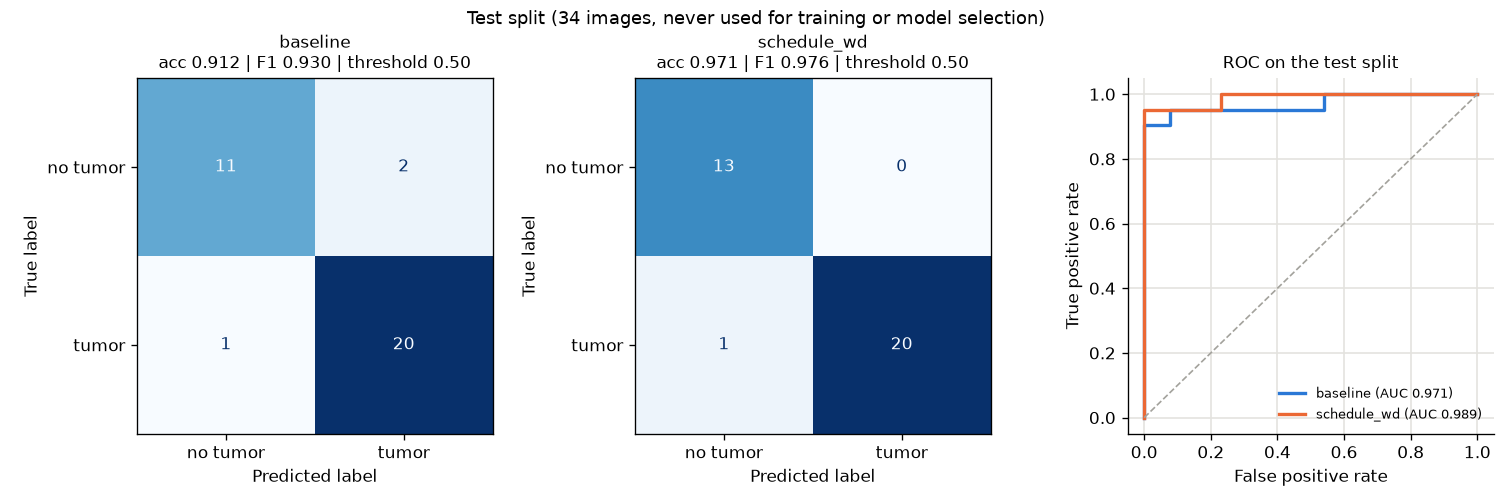
\includegraphics[width=0.74\textwidth]{../results/final/test_comparison.png}
\caption{Matrizes de confusão e curvas ROC no conjunto de teste, nunca usado em treino, seleção de modelo ou escolha de limiar.}
\label{fig:test}
\end{figure*}

\section{Discussão e Ameaças à Validade}

Para a QP1, o \textit{transfer learning} foi o fator determinante: a CNN treinada do zero ficou 0,24 abaixo em AUC e quase não separou as imagens saudáveis, algo esperado com 160 imagens de treino.

Para a QP2, não há evidência de que os ajustes de treino alterem a discriminação: todas as diferenças pareadas têm intervalo que inclui zero, e vitórias e derrotas se dividem quase igualmente. A vantagem de \texttt{schedule\_wd} no teste (0,971 contra 0,912 de acurácia) se resume a duas imagens e está dentro dos intervalos de confiança.

Para a QP3, o limiar ajustado troca pouca sensibilidade por muita especificidade, e de forma instável; uma política de limiar exigiria uma validação maior. Resistem às limitações a vantagem do pré-treino e a equivalência entre as configurações; a estimativa mais confiável do desempenho esperado é a da validação cruzada (AUC próxima de 0,92 e acurácia de 0,85), e não a do teste.

\textit{Validade interna e estatística.} As 15 execuções de cada configuração compartilham imagens de treino, então os ICs pareados são aproximados e tendem a ser estreitos demais. O teste tem 34 imagens, o que explica intervalos de até 0,4 de largura. O \textit{dHash} agrupa apenas quase-duplicatas com \textit{hash} idêntico; cópias recortadas ou com contraste diferente podem ter escapado.

\textit{Validade de construção.} Sem identificação de paciente, não há garantia de que fatias do mesmo paciente fiquem na mesma partição, o que pode inflar todas as métricas. Os rótulos são os das pastas do conjunto, sem revisão por especialista, e não há tipo de tumor nem localização. As classes podem diferir em resolução, sequência e formato do arquivo, o que abre atalhos não relacionados ao tumor.

\textit{Validade externa.} Os dados vêm de uma única coleção, sem metadados de aquisição nem validação externa. Os resultados não indicam uso clínico; no máximo, apoio à triagem após validação em dados independentes.

\section{Conclusão}

Este trabalho comparou uma ResNet-18 pré-treinada e uma CNN treinada do zero na detecção de tumores cerebrais em RM, com deduplicação, divisão por grupos de quase-duplicatas e comparação pareada de quatro configurações de treino por validação cruzada. O pré-treino no ImageNet foi decisivo (AUC de teste de 0,971 contra 0,733), enquanto os ajustes de agendamento, regularização e congelamento ficaram dentro do ruído. O repositório traz ainda ferramentas de segmentação por K-means~\cite{macqueen1967kmeans} e edição manual de máscaras, com três pares imagem/máscara criados. Trabalhos futuros devem usar conjuntos maiores e identificados por paciente, validação externa, calibração das probabilidades e máscaras suficientes para treinar uma rede de segmentação, como a U-Net~\cite{ronneberger2015unet}.

\begin{thebibliography}{99}

\bibitem{swati2019brain}
Z.~N.~K. Swati \emph{et al.}, ``Brain tumor classification for MR images using transfer learning and fine-tuning,'' \emph{Comput. Med. Imaging Graph.}, vol.~75, pp.~34--46, 2019.

\bibitem{deepak2019brain}
S.~Deepak and P.~M. Ameer, ``Brain tumor classification using deep CNN features via transfer learning,'' \emph{Comput. Biol. Med.}, vol.~111, p.~103345, 2019.

\bibitem{kapoor2023leakage}
S.~Kapoor and A.~Narayanan, ``Leakage and the reproducibility crisis in machine-learning-based science,'' \emph{Patterns}, vol.~4, no.~9, p.~100804, 2023.

\bibitem{wen2020alzheimer}
J.~Wen \emph{et al.}, ``Convolutional neural networks for classification of Alzheimer's disease: Overview and reproducible evaluation,'' \emph{Med. Image Anal.}, vol.~63, p.~101694, 2020.

\bibitem{he2016resnet}
K.~He, X.~Zhang, S.~Ren and J.~Sun, ``Deep residual learning for image recognition,'' in \emph{Proc. IEEE CVPR}, 2016, pp.~770--778.

\bibitem{deng2009imagenet}
J.~Deng, W.~Dong, R.~Socher, L.-J. Li, K.~Li and L.~Fei-Fei, ``ImageNet: A large-scale hierarchical image database,'' in \emph{Proc. IEEE CVPR}, 2009, pp.~248--255.

\bibitem{yosinski2014transferable}
J.~Yosinski, J.~Clune, Y.~Bengio and H.~Lipson, ``How transferable are features in deep neural networks?'' in \emph{Advances in NeurIPS}, vol.~27, 2014, pp.~3320--3328.

\bibitem{pedregosa2011sklearn}
F.~Pedregosa \emph{et al.}, ``Scikit-learn: Machine learning in Python,'' \emph{J. Mach. Learn. Res.}, vol.~12, pp.~2825--2830, 2011.

\bibitem{menze2015brats}
B.~H. Menze \emph{et al.}, ``The multimodal brain tumor image segmentation benchmark (BRATS),'' \emph{IEEE Trans. Med. Imag.}, vol.~34, no.~10, pp.~1993--2024, 2015.

\bibitem{kaggle2019brain}
N.~Chakrabarty, ``Brain MRI images for brain tumor detection,'' Kaggle, 2019. [Online]. Available: \url{https://www.kaggle.com/datasets/navoneel/brain-mri-images-for-brain-tumor-detection}

\bibitem{loshchilov2019adamw}
I.~Loshchilov and F.~Hutter, ``Decoupled weight decay regularization,'' in \emph{Proc. ICLR}, 2019.

\bibitem{loshchilov2017sgdr}
I.~Loshchilov and F.~Hutter, ``SGDR: Stochastic gradient descent with warm restarts,'' in \emph{Proc. ICLR}, 2017.

\bibitem{efron1993bootstrap}
B.~Efron and R.~J. Tibshirani, \emph{An Introduction to the Bootstrap}. Chapman \& Hall, 1993.

\bibitem{macqueen1967kmeans}
J.~MacQueen, ``Some methods for classification and analysis of multivariate observations,'' in \emph{Proc. 5th Berkeley Symp. Math. Statist. Probab.}, 1967, pp.~281--297.

\bibitem{ronneberger2015unet}
O.~Ronneberger, P.~Fischer and T.~Brox, ``U-Net: Convolutional networks for biomedical image segmentation,'' in \emph{Proc. MICCAI}, 2015, pp.~234--241.

\end{thebibliography}

\end{document}
